\section{Skid steering drive}

Vehicles equipped with tracks operate on a kinematic principle akin to the differential drive system. 
Each track's speed is individually controlled. 
The height of the track serves as the equivalent of wheel diameter.
This configuration is commonly referred to as Skid Steering. 
However, it requires meticulous calibration and accurate modeling of slippage.
\begin{figure}[H]
    \centering
    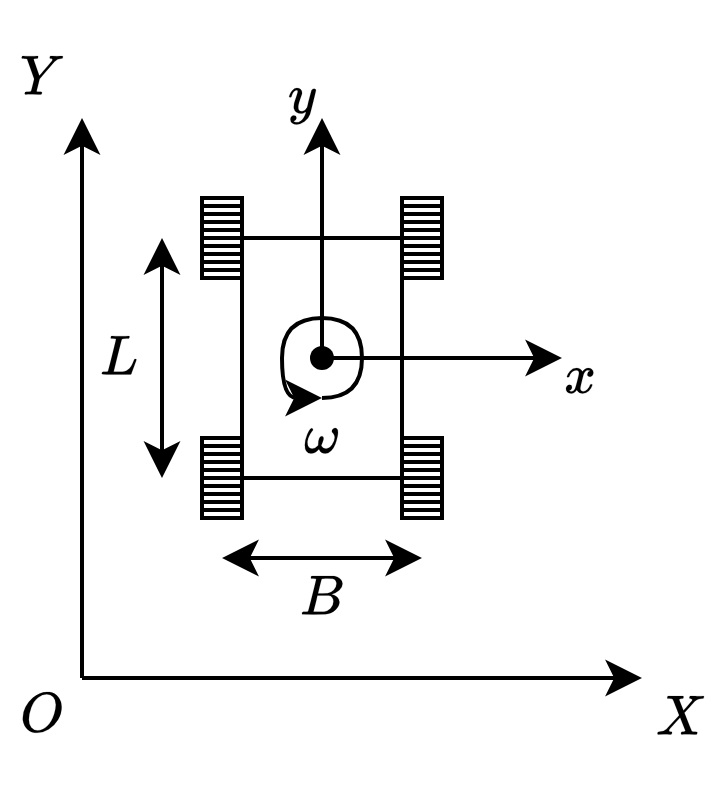
\includegraphics[width=0.3\linewidth]{images/skid.png} 
    \caption{Skid steering drive robot}
\end{figure}
Let's make the following assumptions:
\begin{itemize}
    \item The vehicle's mass is centralized.
    \item All wheels maintain contact with the ground.
    \item Wheels on the same side move at the same speed.
\end{itemize}
While in motion, we encounter multiple Instantaneous Centers of Rotation (ICRs), all sharing the same angular velocity $\omega_z$:
\[\begin{cases}
    \begin{bmatrix}
        v_x \\
        v_y \\
        \omega_z
    \end{bmatrix}= j_\omega\begin{bmatrix}
        \omega_lr \\
        \omega_rr
    \end{bmatrix} \\
    J_\omega=\dfrac{1}{y_l-y_r}\begin{bmatrix}
        -y_r & y_l \\
        x_G & -x_G \\
        -1 & -
    \end{bmatrix}
\end{cases}\]
Assuming symmetry in the robot ($y_0 = y_l = -y_r$), we find:
\[\begin{cases}
    v_x=\dfrac{v_l+v_r}{2} \\
    v_y=0 \\
    \omega_z=\dfrac{-v_l+v_r}{2y_0}
\end{cases}\]
We can determine the instantaneous radius of curvature:
\[\begin{cases}
    R=\dfrac{v_G}{\omega_z}=\dfrac{v_l+v_r}{-v_l+v_r}y_0 \\
    \lambda=\dfrac{v_l+v_r}{-v_l+v_r} \\
    X=\dfrac{2y_0}{B}
\end{cases}\]